%!TeX root = ../main.tex

\section{Development}
Having the time tags in seconds it is sufficient to take a time bin ($T=15\mu s$), and count how many of the dataset ``clicks'' fall inside the range [$nT$, $(n+1)T$], with $n=0,1,2...$ . Plotting on the $x$-axis the number of clicks and on the $y$-axis the number of occurrences inside the time slot, an histogram is derived. The empirical distribution $P(n)$ can be found by dividing the number of clicks $h(n)$ by $N$, number of occurrences (a normalization factor): $P(n)=\dfrac{h(n)}{N}$. The result is shown on figure \ref{fig:still} and \ref{fig:spinning}.
\begin{figure}[H]
    \centering
    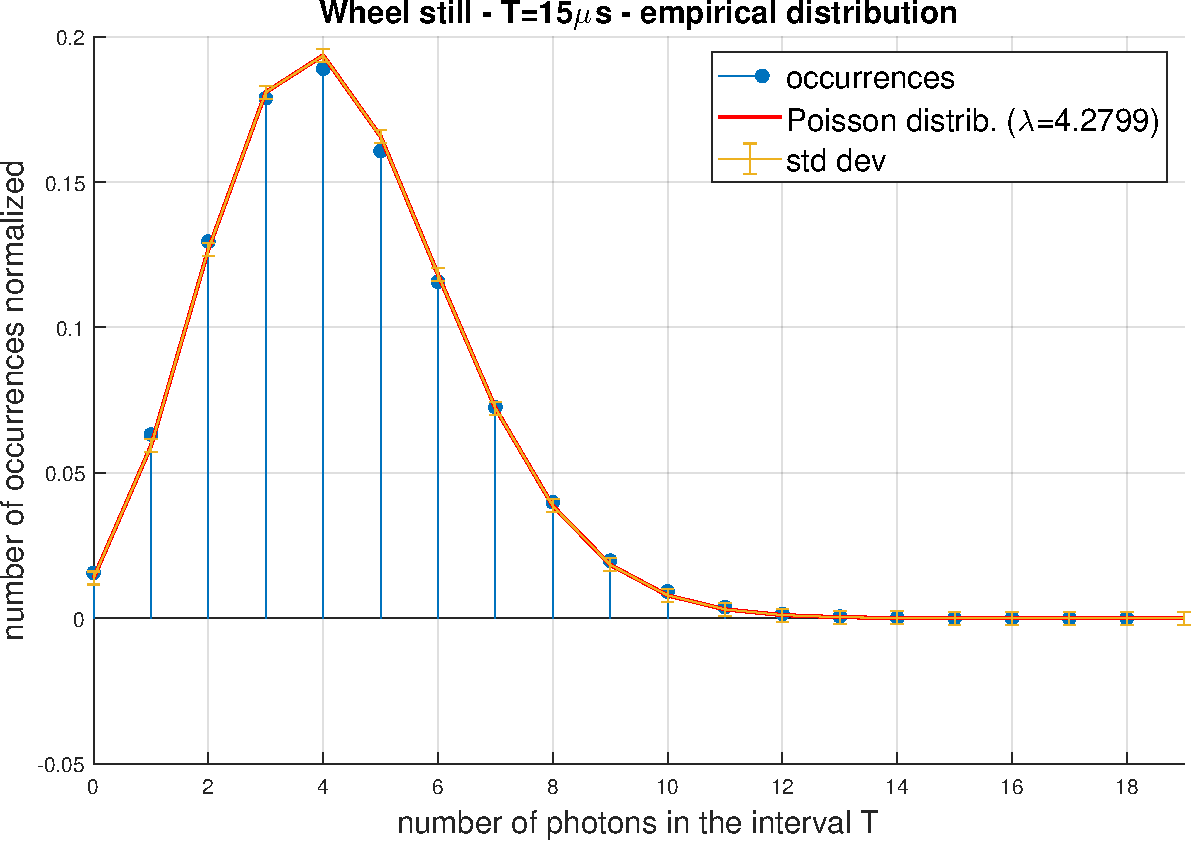
\includegraphics[width=.9\textwidth]{images/Still_Wheel.pdf}
    \caption{Empirical distribution with $T=15\mu s$.}
    \label{fig:still}    
\end{figure}
\begin{figure}[H]
    \centering
    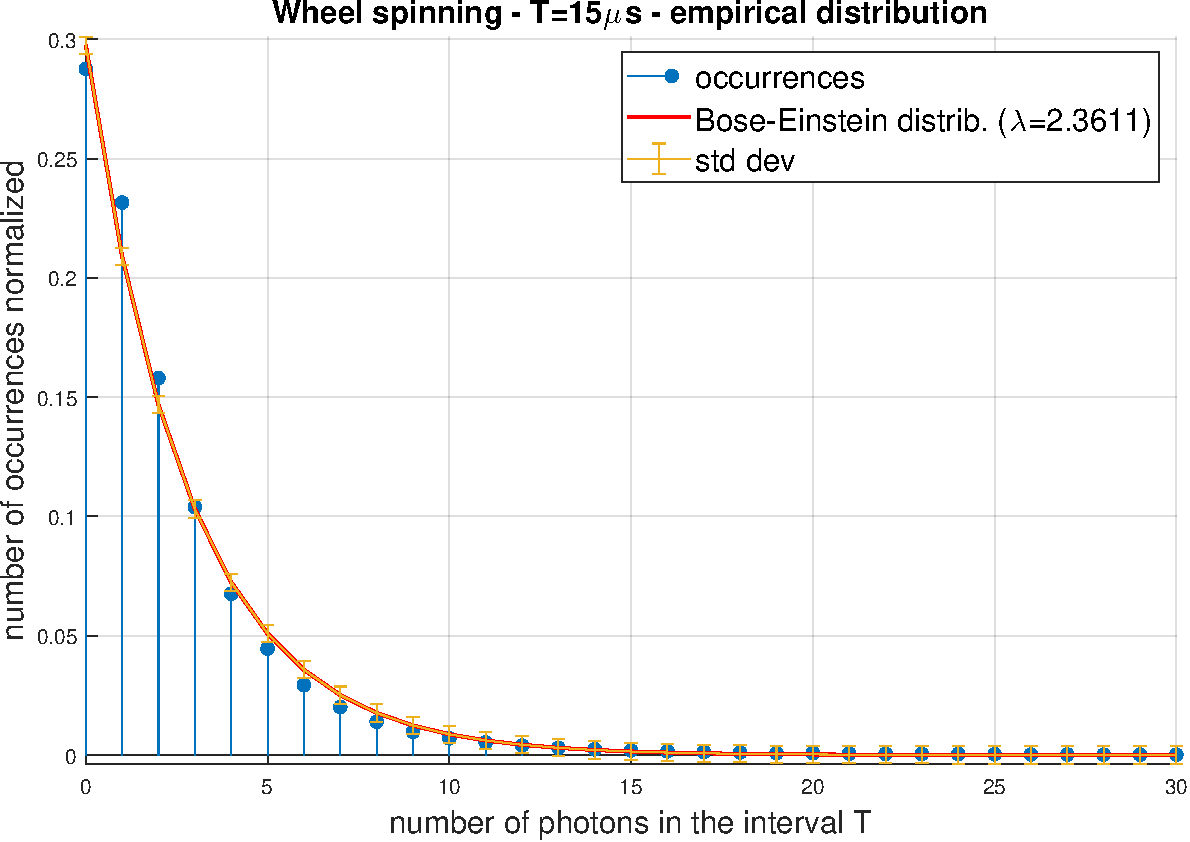
\includegraphics[width=.9\textwidth]{images/Spinning_Wheel.pdf}
    \caption{Empirical distribution with $T=15\mu s$.}
    \label{fig:spinning}    
\end{figure}
In both regimes a plot of the relative distribution is shown for comparison. \\

By changing the size of the time bin, for example to $T=30\mu s$, it is possible to see how the values spread out and the theorical distributions tend to drift away from the empirical data (by increasing the time bin it is increasing the mean and also the variance). The results are shown on figures \ref{fig:still30} and \ref{fig:spinning30}.
\begin{figure}[H]
    \centering
    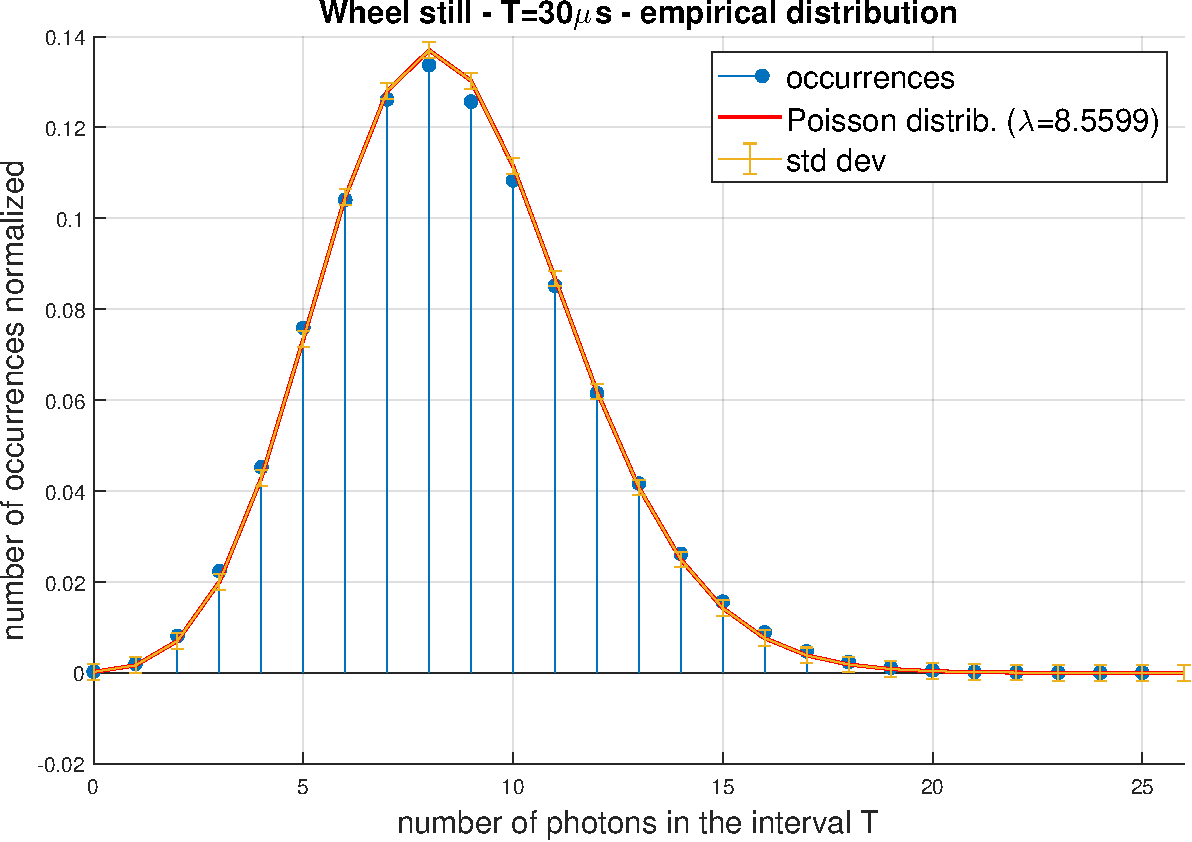
\includegraphics[width=.8\textwidth]{images/Still_Wheel_30.pdf}
    \caption{Empirical distribution with $T=30\mu s$.}
    \label{fig:still30}    
\end{figure}
\begin{figure}[H]
    \centering
    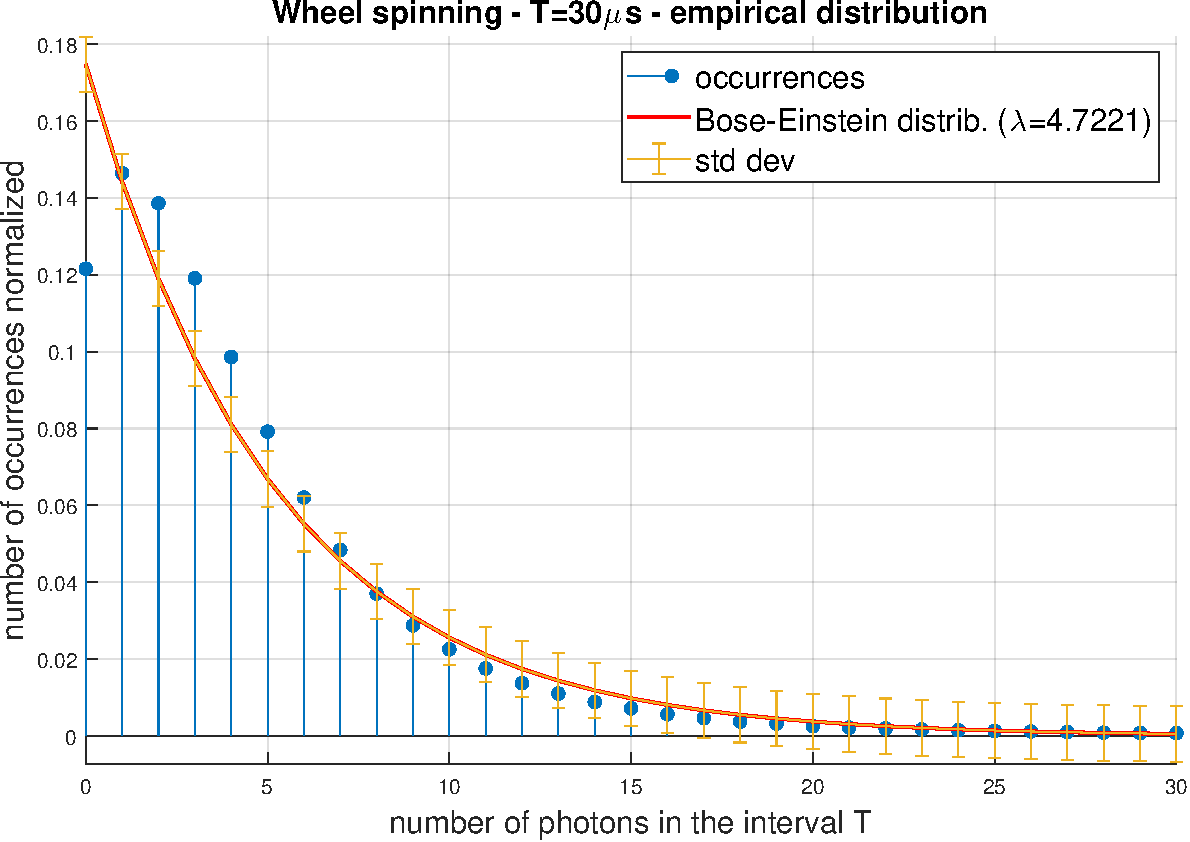
\includegraphics[width=.8\textwidth]{images/Spinning_Wheel_30.pdf}
    \caption{Empirical distribution with $T=30\mu s$.}
    \label{fig:spinning30}    
\end{figure}